
%(BEGIN_QUESTION)
% Copyright 2007, Tony R. Kuphaldt, released under the Creative Commons Attribution License (v 1.0)
% This means you may do almost anything with this work of mine, so long as you give me proper credit

After installing an orifice plate in a flare-line pipe of an oil refinery, operations personnel begin to doubt the accuracy of the flow measurement it provides.  The process fluid going through the flare line varies from hydrogen gas to heavy oils, and its composition continually changes.  Since accurate flow measurement with an orifice plate requires a fluid of {\it known and constant} density, this technique of total flow measurement is doomed.

$$\includegraphics[width=15.5cm]{i01784x01.eps}$$

Flow measurements from the flow transmitters in each unit are far more reliable, because the flare line flow transmitter within each unit may be calibrated for the expected process fluid coming from each unit.  

\vskip 10pt

Determine a way for operations to obtain a reliable total flare flow measurement without having to rely on a single flowmeter in the main flare line.  Hint: it can be done with a {\it computational relay}!

\vskip 20pt \vbox{\hrule \hbox{\strut \vrule{} {\bf Suggestions for Socratic discussion} \vrule} \hrule}

\begin{itemize}
\item{} For those who have already studied flowmeter technology, explain why an orifice-plate flowmeter's accuracy depends on knowing the fluid density.
\item{} This application is an example of an {\it inferred} measurement: obtaining a calculated measurement of some variable that is itself difficult to measure directly.  Identify ways this approach can go wrong, resulting in incorrect inferred values.
\end{itemize}

\underbar{file i01784}
%(END_QUESTION)





%(BEGIN_ANSWER)

$$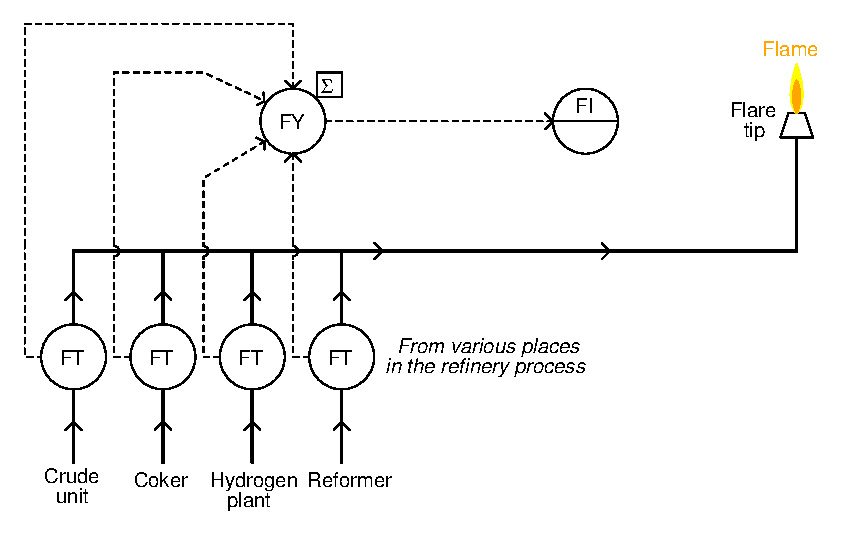
\includegraphics[width=15.5cm]{i01784x02.eps}$$

%(END_ANSWER)





%(BEGIN_NOTES)


%INDEX% Relay, computational: summer relay used in flare flow measurement application

%(END_NOTES)


